%%%%%%%%%%%%%%%%%%%%%%%%%%%%%%%%%%%%%%%%%
% Short Sectioned Assignment
% LaTeX Template
% Version 1.0 (5/5/12)
%
% This template has been downloaded from:
% http://www.LaTeXTemplates.com
%
% Original author:
% Frits Wenneker (http://www.howtotex.com)
%
% License:
% CC BY-NC-SA 3.0 (http://creativecommons.org/licenses/by-nc-sa/3.0/)
%
%%%%%%%%%%%%%%%%%%%%%%%%%%%%%%%%%%%%%%%%%

%----------------------------------------------------------------------------------------
% PACKAGES AND OTHER DOCUMENT CONFIGURATIONS
%----------------------------------------------------------------------------------------

\documentclass[paper=a4, fontsize=11pt,numbers=endperiod]{scrartcl} % A4 paper and 11pt font size

\usepackage[T1]{fontenc} % Use 8-bit encoding that has 256 glyphs
%\usepackage{fourier} % Use the Adobe Utopia font for the document - comment this line today return to the LaTeX default
\usepackage[english]{babel} % English language/hyphenation
\usepackage{amsmath,amsfonts,amsthm} % Math packages

\usepackage[utf8]{inputenc} % Needed to support swedish "åäö" chars
\usepackage{titling} % Used to re-style maketitle

\usepackage{lipsum} % Used for inserting dummy 'Lorem ipsum' text into the template

\usepackage{sectsty} % Allows customizing section commands
\allsectionsfont{\normalfont} % Make all sections the default font

% Local packages:
\usepackage{enumerate}
\usepackage[usenames,dvipsnames]{color}
\usepackage{tabularx}
\usepackage{fancyvrb}
\DefineShortVerb{\|}
\usepackage{hyperref}
\usepackage{url}
\usepackage[parfill]{parskip}   % Sets newlines between paragraphs
\usepackage{algorithm2e} % Used for Pseudocode
\providecommand{\abs}[1]{\lvert#1\rvert} % \abs{x+y} produces |x+y|
\usepackage{graphicx}
\DeclareGraphicsExtensions{.png,.jpg}
\usepackage{sectsty}





\usepackage{fancyhdr} % Custom headers and footers
\pagestyle{fancyplain} % Makes all pages in the document conform to the custom headers and footers

% Header with additional info
% \fancyhead[L]{\small{Gustaf Lindstedt - \href{mailto:glindste@kth.se}{\color{RoyalBlue}\nolinkurl{glindste@kth.se}} - 910301\\Martin Runelöv - \href{mailto:mrunelov@kth.se}{\color{RoyalBlue}\nolinkurl{mrunelov@kth.se}} - 900330-5738}}
% Simple header
\fancyhead[L]{\small{Gustaf Lindstedt\\Martin Runelöv}} % 


\fancyfoot[L]{} % Empty left footer
\fancyfoot[C]{} % Empty center footer
\fancyfoot[R]{\thepage} % Page numbering for right footer
\renewcommand{\headrulewidth}{0pt} % Remove header underlines
\renewcommand{\footrulewidth}{0pt} % Remove footer underlines
\setlength{\headheight}{23.0pt} % Customize the height of the header
\fancyhfoffset[L]{10mm}% slightly less than 0.25in

\numberwithin{equation}{section} % Number equations within sections (i.e. 1.1, 1.2, 2.1, 2.2 instead of 1, 2, 3, 4)
\numberwithin{figure}{section} % Number figures within sections (i.e. 1.1, 1.2, 2.1, 2.2 instead of 1, 2, 3, 4)
\numberwithin{table}{section} % Number tables within sections (i.e. 1.1, 1.2, 2.1, 2.2 instead of 1, 2, 3, 4)


\allsectionsfont{\bfseries}

\setlength\parindent{0pt} % Removes all indentation from paragraphs - comment this line for an assignment with lots of text


\posttitle{\par\end{center}} % Remove space between author and title
%----------------------------------------------------------------------------------------
% TITLE SECTION
%----------------------------------------------------------------------------------------

\title{ 
\huge Project 2 - Euclidean TSP \\ % The assignment title
\vspace{10pt}
\normalfont \normalsize 
\textsc{DD2440 - Advanced algorithms } \\ [25pt] % 
}

\author{Gustaf Lindstedt \\ glindste@kth.se \\ 910301-2135 \and Martin Runelöv \\ mrunelov@kth.se \\ 900330-5738}

\date{\vspace{8pt}\normalsize\today} % Today's date or a custom date

\begin{document}

\maketitle % Print the title


%-------------------------------------------------------------------------------
% SECTION 1
%-------------------------------------------------------------------------------
\hspace{0pt}\\
\section*{Statement of collaboration}
All of the research was done together, and the report was written together.
Gustaf implemented the initial 2-opt, and Martin implementented the initial 2.5-opt.
Gustaf did the initial satellite lists and neighbour lists. Gustaf reworked 2-opt to work with satellite lists.
Martin reworked 2.5-opt to work with satellite lists, and reworked Nearest Neighbour and 2.5-opt to work with with the neighbour lists.

\section{Introduction}

% heh orkade inte ha ett intro direkt med underrubrik.
This project was done as part of the course \emph{Advanced Algorithms} at the Royal Instityte of Technology, KTH.

\subsection{Problem}

The traveling salesman problem (TSP) is famous in both theoretical computer science and in operations research. It asks the following question: 

\begin{center}
    \emph{Given a list of cities and the distance between each pair of cities, what is the shortest possible route that visits each city exactly once and returns to the origin city?}
\end{center}

Our problem consists of finding such a tour in Euclidean space. This means that a distance from city A to city B is equal to the distance from B to A, and that the triangle inequality holds.

%-------------------------------------------------------------------------------
% SECTION 2
%-------------------------------------------------------------------------------
\section{Algorithms}

\subsection{Nearest neighbour}

\subsection{Local optimization algorithms}
When a tour has been calculated, we can perform local optimization by examining parts of the tour.

\subsubsection{2-opt}
Swap two arcs.

\subsubsection{2.5-opt}
2.5-opt, also known as 2h-opt, works as follows:

Pick one city B. B is currently between cities A and C. Try to move B to between any other two cities D and E such that the total distances becomes shorter. With $d$ being the distance function for two cities, we are looking for cities A-E such that the following is true:
\[
    \underbrace{d(A,B) + d(B,C) + d(D,E)}_\text{Old distances}\; > \;\underbrace{d(A,C) + d(D,B) + d(B,E)}_\text{New distances}
\]

The below image illustrates the concept:

\begin{center}
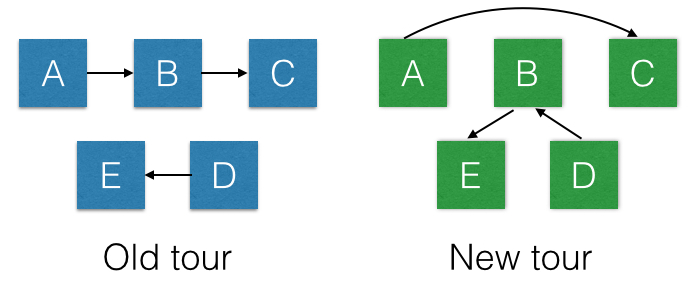
\includegraphics[scale=0.4]{25opt}
\end{center}



%----------------------------------------------------------------------------------------
% SECTION 3
%----------------------------------------------------------------------------------------
\section{Implementation}
The program was implemented in the C programming language.


\subsection{Satellite lists}
In order to effectively perform the local optimizations a specialized data structure is required. In particular, we need to optimize operations such as reversing a subtour, and moving a city. To move a city, we need a structure that has tour positions that are independent from other parts of the tour. This can be achieved with a doubly linked list since it allows us to easily move individual cities. However, to optimize reversal of a subtour we need something called \emph{satellite lists}. They use ...etc etc.

\begin{center}
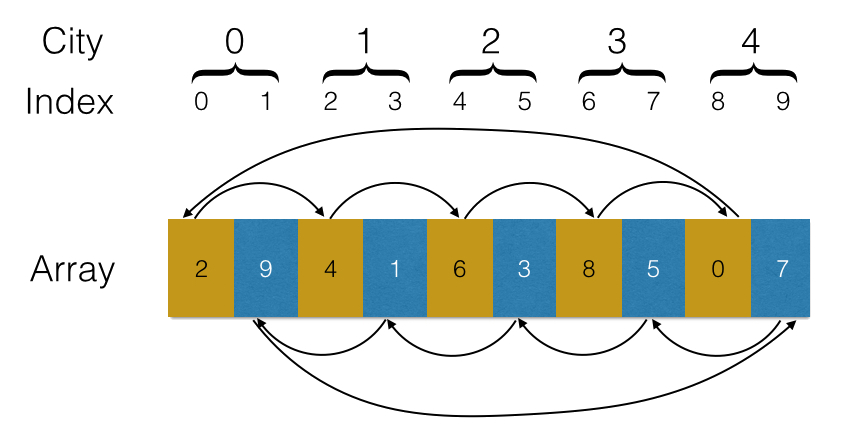
\includegraphics[scale=0.3]{satellite}
\end{center}



%------------------------------------------------------------------------------
%   SECTION 4
%-------------------------------------------------------------------------------

\section{Results}

    \begin{tabular}{|c|c|c|c|c|}
    \hline
    \textbf{Algorithm} & \textbf{Score} \\ \hline
    Nearest Neighbour & 3 \\ \hline
    NN + 2-opt & 19 \\ \hline
    NN + 2.5-opt & 25 \\ \hline
    \end{tabular}
    \hspace{10pt}


\section{Discussion}

% Nåt generellt om projektet kanske. 

% Nåt om satellite antar jag. Dom är lite dryga.
All concepts and algorithms used are relatively easy to understand, but they became harder to implement with satellite lists. The satellite lists required us to think carefully when changing the tour.

% Avsluta med något om hur nöjda vi är?



%----------------------------------------------------------------------------------------
% REFERENCES
%----------------------------------------------------------------------------------------
\newpage
\begin{thebibliography}{9}

% TODO TODO TODO TODO TODO TODO TODO  TODO TODO TODO TODO  TODO TODO TODO TODO 
% INSERT GODDAMN DATES!
\bibitem{algnotes} Notes for the course advanced algorithms - \url{http://www.nada.kth.se/~johanh/algnotes.pdf} <insert date here!>
 
\end{thebibliography}

\end{document}
